La capa de convolución es uno de los componentes fundamentales en una red neuronal convolucional. Esta capa realiza operaciones de convolución en la entrada, lo que permite que la red aprenda características relevantes de los datos, como patrones visuales en una entrada de imágenes.

\textbf{Filtro}

La capa de convolución utiliza filtros (también llamados kernels) que son matrices pequeñas (por ejemplo, 3x3 o 5x5) que se deslizan sobre la entrada. Estos filtros son los parámetros que se aprenden durante el entrenamiento de la red. Durante la fase de entrenamiento, la red aprende automáticamente los valores óptimos para los filtros convolucionales que maximizan su capacidad para reconocer patrones relevantes en los datos de entrada. Este proceso se lleva a cabo de la siguiente manera:
 
 \begin{itemize}
	\item Inicialización de pesos: Al inicio, los pesos de los filtros se inicializan de forma aleatoria o utilizando estrategias específicas.
	
	\item Forward propagation: Durante la fase de forward propagation, los datos se propagan a través de la red. En las capas de convolución, los filtros se aplican a las entradas para generar mapas de características. 
	
	\item Cálculo de la pérdida: Se compara la salida de la red con las etiquetas reales (durante el entrenamiento supervisado) utilizando una función de pérdida, que mide qué tan bien la red está prediciendo las etiquetas.
	
	\item Backpropagation: Utilizando la función de pérdida, se calcula el gradiente de esta función con respecto a los pesos de la red, incluyendo los filtros en las capas de convolución. La retropropagación se utiliza para determinar cómo los pesos deben ajustarse para minimizar la pérdida.
	
	\item Actualización de pesos: Los pesos, incluidos los filtros, se actualizan en la dirección opuesta al gradiente para reducir la pérdida. Se utiliza un algoritmo de optimización, como el descenso de gradiente estocástico (SGD), para realizar estas actualizaciones.

	\item Iteración: Este proceso se repite para múltiples iteraciones (épocas) a medida que la red continúa refinando los pesos y los filtros para mejorar su capacidad de generalización en los datos de entrenamiento.
\end{itemize}

\textbf{Operación de convolución}

En términos generales, la convolución es una operación donde se  aplica un filtro o núcleo a regiones pequeñas de la entrada de la red convolucional, desplazándose secuencialmente. Esto involucra la multiplicación elemento por elemento entre el filtro y la sección correspondiente de la entrada. Estos productos se suman para generar un único valor en una nueva matriz, conocida como mapa de características o feature map, ver Figura \ref{fig:an10}

\begin{figure}[h!]
	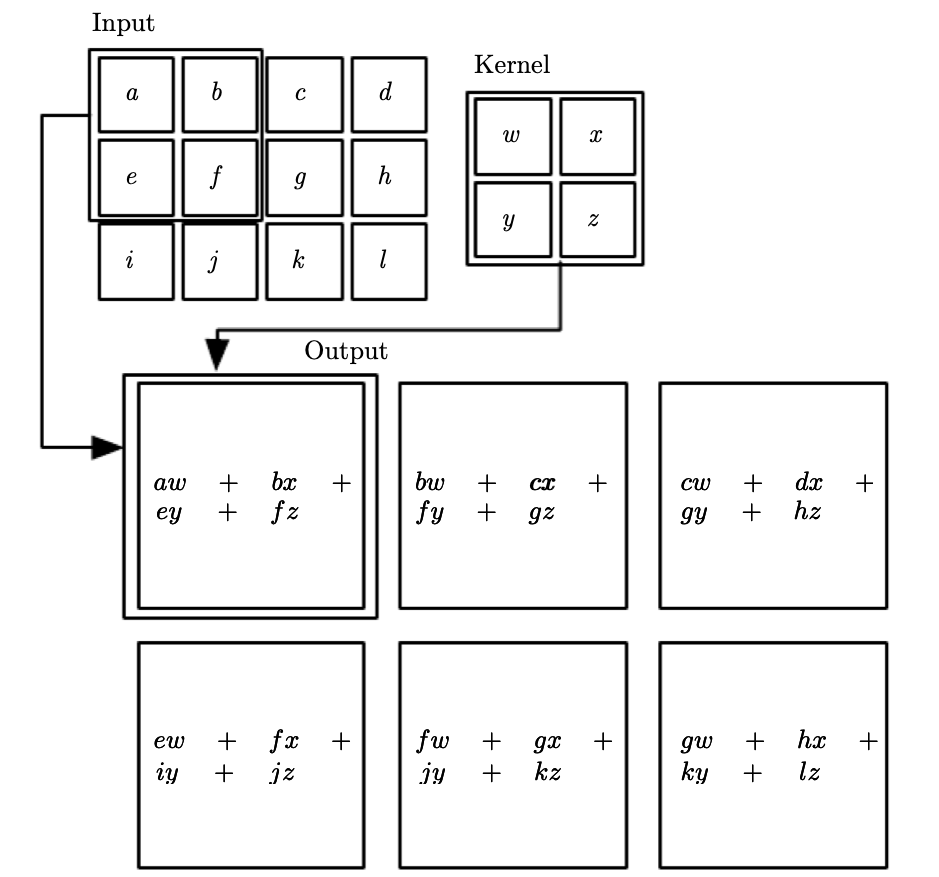
\includegraphics[width=0.6\textwidth]{capitulo2/figuras/an10.png}
	\caption[Convolución valida 2-D sin kernel volteado]{Convolución valida 2-D sin kernel volteado
		\\\textit{Fuente: Extraído de} \protect\cite[p. 334]{goodfellow2016deep}}
	\label{fig:an10}
\end{figure}

Comúnmente, la operación de convolución se representa con un asterisco. ver ecuación \ref{eq:e16}.

\begin{equation} \label{eq:e16} 
	s(i,j)=(I\ast K)
\end{equation}

Por ejemplo, en el caso de que se use un vector bidimensional I como entrada y un núcleo bidimensional K, la operación de convolución sería equivalente a la ecuación \ref{eq:e17} :

\begin{equation} \label{eq:e17} 
	S(i,j)=(I\ast K)(i,j)=\sum_{m}^{}\sum_{n}^{}I(m,n)K(i-m,j-n)
\end{equation}

Si se quiere invertir el núcleo, en el dado caso que se pueda aprovechar la conmutatividad de la operación de convolución, su representación se encuentra en la ecuación \ref{eq:e18}. Donde la  diferencia principal de la ecuación \ref{eq:e17} radica en el orden de los índices de desplazamiento de las variables de la convolución. Ya que a medida que m y n aumentan, los índices de la entrada aumentan, mientras que los de los índices del núcleo disminuyen.

\begin{equation} \label{eq:e18} 
	S(i,j)=(K\ast I)(i,j)=\sum_{m}^{}\sum_{n}^{}I(i-m,j-n)K(m,n)
\end{equation}

Muchas bibliotecas de redes neuronales implementan una función relacionada llamada correlación cruzada como muestra la ecuación \ref{eq:e19}, qué es lo mismo que la convolución pero sin invertir el núcleo.
\begin{equation} \label{eq:e19} 
	(I\ast K)(i,j)=\sum_{m}^{}\sum_{n}^{}I(i+m,j+n)K(m,n)
\end{equation}


La operación de convolución es un paso más para generar el necesario mapa de características, en el caso de que la entrada sea texto se  aplica el filtro w a una ventana de palabras  para crear una nueva característica. Por ejemplo, una característica $c_i$ se genera mediante la mediante la ecuación :

\begin{equation} \label{eq:e20} 
	c_i = f(\mathbf{w}\cdot \mathbf{x}_{i:i+h-1} + b)
\end{equation}
 

	
En la ecuación \ref{eq:e20} $b$ representa el término de sesgo, y $f$ es una función no lineal. El filtro en este caso representado por $w$ se emplea en cada ventana posible de palabras $x_i:i+h-1$ en la oración para generar un mapa de características $c=[c_1,c_2,\ldots,c_{n-h+1}]$. Es decir que, una vez que la entrada pasa por la capa de convolución y se le suma el sesgo, entonces se le aplicará una funcion de activacion para generar salidas no lineales a la entrada para finalmente aplicar la operación de pooling que se detallara más adelante.

 \textbf{Padding}
 
 El padding (relleno) se refiere a agregar valores adicionales alrededor de los bordes de la entrada antes de aplicar el filtro de convolución. Este proceso se utiliza para controlar el tamaño de la salida después de la operación de convolución.
Cuando se aplica un filtro a una entrada en una CNN, el tamaño de la salida se reduce debido a que el filtro no puede aplicarse a los bordes de la entrada. El padding resuelve este problema agregando filas y columnas adicionales de ceros o valores específicos alrededor de la entrada. Estos valores adicionales actúan como un ``borde'' alrededor de la entrada y permiten que el filtro se aplique a las regiones de los bordes de manera más efectiva.

Hay tres tipos comunes de padding: 

\begin{itemize}

	\item Padding ``same'' agrega suficientes filas y columnas de ceros alrededor de la entrada para asegurar que la salida tenga el mismo tamaño que la entrada original después de la convolución. ``En este caso, la red puede contener tantas capas convolucionales como el hardware disponible pueda soportar, ya que la operación de convolución no modifica las posibilidades arquitectónicas disponibles para la siguiente capa.''\cite[p. 350]{goodfellow2016deep}. Sin embargo, los elementos de la entrada cerca del borde influyen en menos elementos de salida que los elementos de la entrada cerca del centro, esto puede hacer que los elementos del borde estén algo subrepresentados en el modelo.
	
	\item Padding ``valid'' no agrega ningún relleno y permite que el filtro se aplique solo a las regiones donde el filtro y la entrada se superponen completamente, lo que produce una salida más pequeña que la entrada. ``Si la imagen de entrada tiene un ancho $m$ y el núcleo tiene un ancho $k$, la salida será de ancho $m - k + 1$. La tasa de esta contracción puede ser dramática si los núcleos utilizados son grandes.'' \cite[p. 350]{goodfellow2016deep}.
	
	\item Padding ``full'' se agregan ceros de tal manera que cada elemento en el borde sea visitado k veces, en cada dirección por el núcleo de convolución. Esto se traduce en una  salida que tiene un ancho mayor  que la entrada original, generalmente $m + k - 1$. En esta configuración, los elementos en los bordes de la  de salida están influenciados por menos elementos de la  entrada que los elementos más cercanos al centro. Esta disparidad puede dificultar que un único núcleo funcione de manera óptima en todas las posiciones del mapa de características.
	
\end{itemize}

El uso de padding en una CNN es crucial para controlar el tamaño de la salida y preservar la información en los bordes de la entrada durante la convolución. Esto es especialmente importante cuando se desean mantener detalles espaciales importantes en la imagen o secuencia de entrada. ``Por lo general, la cantidad óptima de relleno de ceros (en términos de precisión de clasificación del conjunto de pruebas) se encuentra en algún lugar entre la convolución ``válid'' y  ``same''.''\cite[p.350]{goodfellow2016deep}.

\textbf{Stride}

El stride (paso) se refiere a la cantidad de desplazamiento que se aplica al filtro convolucional a medida que se mueve a lo largo de la entrada. Un stride mayor significa que el filtro se mueve en incrementos más grandes, lo que resulta en una reducción del tamaño espacial de la salida. Por otro lado, un stride menor permite un solapamiento más grande entre las operaciones de convolución sucesivas y produce una salida con mayor tamaño espacial.
El ajuste del stride en una CNN puede influir en la dimensionalidad de la salida de cada capa convolucional, lo que a su vez puede afectar el número de parámetros y la información espacial conservada en la red. El stride se elige considerando la complejidad del problema, la dimensionalidad de la entrada y las características que se desean extraer de los datos.


	